\textbf{$\ket{1}$}\vspace{.2cm}

\textcolor{bibi}{Usando estado inicial}\vspace{.2cm}

\begin{quote}
    \begin{minted}[fontsize=\small, linenos, frame=single]{python}
estado_inicial = [0,1]
circuito1 = QuantumCircuit(1)
circuito1.initialize(estado_inicial,0)
circuito1.measure_all()
circuito1.draw('mpl')
    \end{minted}
    \vspace{.3cm}
    \begin{center}
        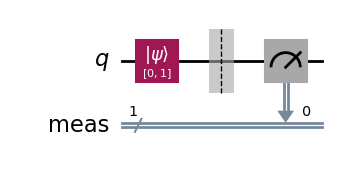
\includegraphics[height=3.3cm]{src/Img/1.1.png}
    \end{center}

    Este es bastante sencillo lo único que hay que hacer es utilizar el estado inicial
    $\ket{1}$ que se hace en la linea 1 dándole $\alpha=0, \beta=1$. Si medimos la salida nos
    dara: 
    \vspace{.5cm}

    \begin{center}
        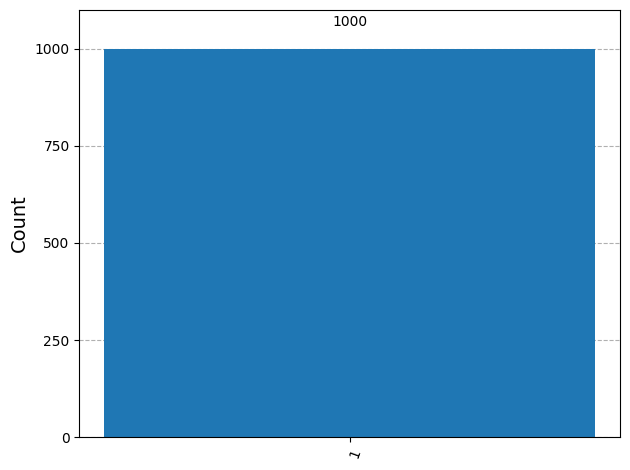
\includegraphics[height=6cm]{src/Img/1.1.r.png}
    \end{center}
\end{quote}
\newpage
